\section{Неделя I}

\subsection*{№1}

Рассмотрим уравнение на $G(t)$
\begin{equation}
    (\partial_t + \gamma) G(t) = \delta(t),
    \label{w1_eq1}
\end{equation}
с учетом принципа причинности $g(t<0) = 0$. 

При $t > 0$ $\delta(t) = 0$,  так что
\begin{equation*}
    \partial_t G(t) = - \gamma G(t),
    \hspace{0.5cm} \Rightarrow \hspace{0.5cm}
    G(t) = A \exp(- \gamma t).
\end{equation*}
Проинтегрируем уравнение \eqref{w1_eq1} от $-\varepsilon$ до $\varepsilon$:
\begin{equation*}
    G'(\varepsilon) - \cancel{G'(-\varepsilon)} + \cancel{\int_{-\varepsilon}^{\varepsilon} \gamma G(t) \d t } = \int \delta(t) \d t = 1,
    \hspace{0.5cm} \Rightarrow \hspace{0.5cm}
    G'(\varepsilon) = 1, 
    \hspace{0.5cm} \Rightarrow \hspace{0.5cm}
    A = 1.
\end{equation*}
Таким образом, искомая функция Грина $G(t)$:
\begin{equation*}
    G(t) = \theta(t) \cdot \exp\left(- \gamma t\right),
\end{equation*}
где $\theta(t)$ обеспечивает $G(t) = 0$ при $t<0$.




\subsection*{№2}

Рассмотрим уравнение, вида
\begin{equation*}
    (\partial_t^2 + \omega^2) \varphi(t) = g(t),
    \hspace{5 mm}   
    g(t) = \left\{\begin{aligned}
        &0, &t\notin [0, \tau]; \\
        &- \tfrac{v}{\tau l}, &t \in [0, \tau], \\
    \end{aligned}\right.
    \label{w1_t2}
\end{equation*}
с нулевым начальным условием $\varphi(t<0)=0$.
Функция Грина $G(t)$ для оператора $(\partial_t^2 + \omega^2)$ равна\footnote{
    Конспект, уравнение (1.11).
} 
\begin{equation*}
    G(t) = \theta(t) \frac{1}{\omega} \sin(\omega t).
\end{equation*}
Далее найдём вид $\varphi(t)$ при $t < \tau$ (красная линия рис. \ref{fig:I2}):
\begin{equation*}
    \varphi(t < \tau) = \frac{1}{\omega} \int_{-\infty}^{t} \sin \omega(t-s) \ g(s) \d t = \frac{1}{\omega} \int_0^t \sin \omega(t-s) \frac{v}{2l} \d (t-s) = 
    \frac{v}{l \tau} \frac{1}{\omega^2} \left(
        \cos(\omega t) - 1
    \right).
\end{equation*}

\begin{figure}[ht]
    \centering
    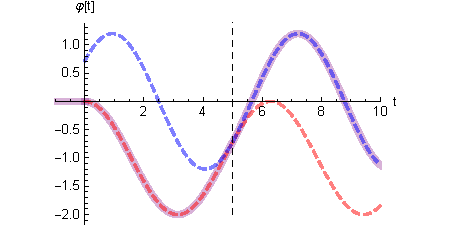
\includegraphics[width=0.5\textwidth]{figures/T2.pdf}
    \caption{Сшивка решений в I.2}
    \label{fig:I2}
\end{figure}

Теперь решим\footnote{
    Конспект, уравнение (1.12).
}  задачу Коши с начальным условием при $t = \tau$, введя переменную $T = t-\tau$:
\begin{equation*}
    \varphi(T) = \varphi(t-\tau) = \dot{\varphi}(\tau) G(t-\tau) + \varphi(\tau) \dot{G}(t-\tau) + 0 = 
    \frac{v}{lt} \frac{1}{\omega^2} \left(
        \cos \omega t - \cos \omega(t-\tau)
    \right).
\end{equation*}
 получая синюю кривую на рис. \ref{fig:I2}.

 Итого, решение уравнения \eqref{w1_t2} (фиолетовая кривая, рис \ref{fig:I2}):
 \begin{equation*}
     \varphi(t) = \frac{v}{l \tau} \frac{1}{\omega^2}\left\{\begin{aligned}
        &0
        , &t < 0; \\
        & \cos \omega t - 1
        , &t \in [0, \tau]; \\
        & \cos \omega t - \cos \omega(t-\tau)
        , &t > \tau. \\
     \end{aligned}\right.
 \end{equation*}


 \subsection*{№3}


 Найдём значение интеграла, вида
 \begin{equation*}
     I_1= \int_{-\infty}^{+\infty} \frac{1}{(x^2 + a^2)^2} \d x.
 \end{equation*}
 Заметим, что уравнение $z^2 + a^2 = 0$ имеет корни в $z_{1, 2} = a^{\pm i \pi/2}$, тогда
 \begin{equation*}
     I_1 = 2 \pi i \cdot \text{res}_{z_1} = 2 \pi i 
     \lim_{z \to z_1} \cdot \left(
        \frac{1}{(z- z_2)^2}
     \right)' = -4 \pi i \cdot \lim_{z \to z_1} \left(
        \frac{1}{(z-z_2)^3}
     \right) = - 4 \pi i \frac{1}{(2 i a)^3} = \frac{\pi}{2 a^3}.
 \end{equation*}

